\documentclass[a4paper]{article}
\usepackage{graphicx} % Required for inserting images
\usepackage{float} % Para agregar imagen en el lugar
\usepackage{tikz} % Insertar gráficos
\usepackage{amsmath}% Para usar ecuaciones
\usepackage{siunitx} % para angulos
\usepackage{wrapfig} % Imagen con texto al lado
\usepackage{caption}
\usepackage{subcaption}
\usepackage[a4paper, total={6in, 9in}]{geometry}


%-------------------------------
\begin{document}

\section{Ecuaciones de latitud}
%----------SUR-----------
\begin{figure}[H]
    \centering
    \begin{subfigure}{0.3\textwidth}
        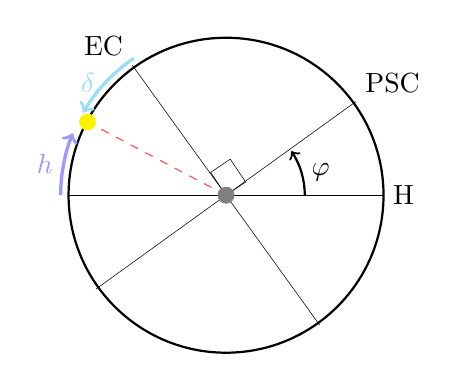
\begin{tikzpicture}
            % Circunferencia
            \draw[black, thick] (0,0) circle (2);
            
            % Rectas / Líneas
            \draw[black, very thin] (-2, 0) -- (2, 0) node[anchor=west]{H};
            \draw[black, very thin] (-1.65, -1.19) -- (1.65, 1.19) node[anchor=south west]{PSC};
            \draw[black, very thin]  (1.19, -1.65) -- (-1.19, 1.65)  node[anchor=south east]{EC};
            % Línea roja
            \draw[red!70, dashed] (0,0) -- (-1.76, 0.93);
        
            % Arcos
            % Declinación
            \draw[cyan!40, very thick, ->] (-1.17, 1.74) arc (124:150:2.1) node[midway, left]{$\delta$};
            % Altura h
            \draw[blue!40, very thick, ->] (-2.1, 0) arc (180:158:2.1) node[midway, left]{$h$};
            \draw[black, thick, ->] (1, 0) arc (0:34:1) node[midway, right]{$\varphi$};
            
            % % Cuadrados
            \draw[black, very thin, rotate around={34:(0,0)}] (0,0) rectangle (0.3, 0.35);
        
            % % Puntos
            \filldraw[fill=black!50, draw=black!50] (0,0) circle (0.1);
            % Estrella a 152º
            \filldraw[fill=yellow, draw=yellow] (-1.76, 0.93) circle (0.1); 
        \end{tikzpicture}
        \caption{$\varphi = h + \delta - \ang{90}$}
    \end{subfigure}
    \hspace{0.1cm}
    \hfill
    \begin{subfigure}{0.3\textwidth}
        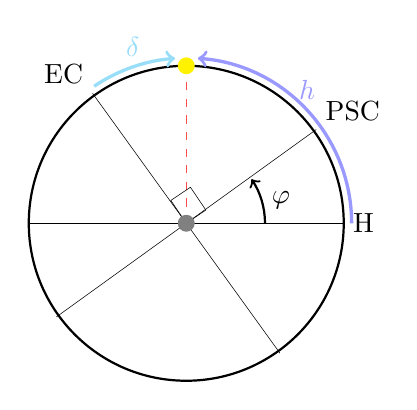
\begin{tikzpicture}
            % Circunferencia
            \draw[black, thick] (0,0) circle (2);
            
            % Rectas / Líneas
            \draw[black, very thin] (-2, 0) -- (2, 0) node[anchor=west]{H};
            \draw[black, very thin] (-1.65, -1.19) -- (1.65, 1.19) node[anchor=south west]{PSC};
            \draw[black, very thin]  (1.19, -1.65) -- (-1.19, 1.65)  node[anchor=south east]{EC};
            % Línea roja
            \draw[red!70, dashed] (0,0) -- (0, 2);
        
            % Arcos
            % Declinación
            \draw[cyan!40, very thick, ->] (-1.17, 1.74) arc (124:94:2.1) node[midway, above]{$\delta$};
            % Altura h
            \draw[blue!40, very thick, ->] (2.1, 0) arc (0:86:2.1) node[midway, above]{$h$};
            \draw[black, thick, ->] (1, 0) arc (0:34:1) node[midway, right]{$\varphi$};
            
            % % Cuadrados
            \draw[black, very thin, rotate around={34:(0,0)}] (0,0) rectangle (0.3, 0.35);
        
            % % Puntos
            \filldraw[fill=black!50, draw=black!50] (0,0) circle (0.1);
            % Estrella a 90º
            \filldraw[fill=yellow, draw=yellow] (0, 2) circle (0.1); 
        \end{tikzpicture}
        \caption{$\varphi = \ang{90} + \delta - h$}
    \end{subfigure}
    % \hspace{0.05cm}
    \hfill
    \begin{subfigure}{0.3\textwidth}
        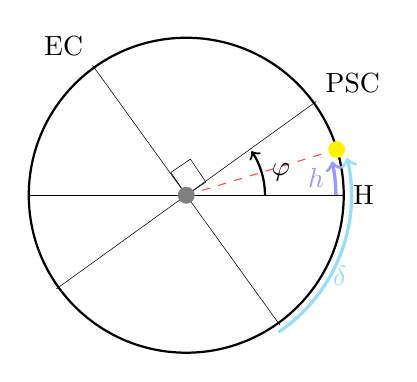
\begin{tikzpicture}
            % Circunferencia
            \draw[black, thick] (0,0) circle (2);
            
            % Rectas / Líneas
            \draw[black, very thin] (-2, 0) -- (2, 0) node[anchor=west]{H};
            \draw[black, very thin] (-1.65, -1.19) -- (1.65, 1.19) node[anchor=south west]{PSC};
            \draw[black, very thin]  (1.19, -1.65) -- (-1.19, 1.65)  node[anchor=south east]{EC};
            % Línea roja
            \draw[red!70, dashed] (0,0) -- (1.91, 0.58);
        
            % Arcos
            % Declinación
            \draw[cyan!40, very thick, ->] (1.17, -1.74) arc (-56:13:2.1) node[midway, below]{$\delta$};
            % Altura h
            \draw[blue!40, very thick, ->] (1.9, 0) arc (0:13:1.9) node[midway, left]{$h$};
            \draw[black, thick, ->] (1, 0) arc (0:34:1) node[midway, right]{$\varphi$};
            
            % % Cuadrados
            \draw[black, very thin, rotate around={34:(0,0)}] (0,0) rectangle (0.3, 0.35);
        
            % % Puntos
            \filldraw[fill=black!50, draw=black!50] (0,0) circle (0.1);
            % Estrella a 17º
            \filldraw[fill=yellow, draw=yellow] (1.91, 0.58) circle (0.1); 
        \end{tikzpicture}
        \caption{$\varphi = \delta - h - \ang{90}$}
    \end{subfigure}  
    \caption{Ecuaciones de latitud en hemisferio sur}
    \label{fig:lat-hemisferio-sur}
\end{figure}


%----------NORTE-------------
\begin{figure}[H]
    \centering
    \begin{subfigure}{0.3\textwidth}
        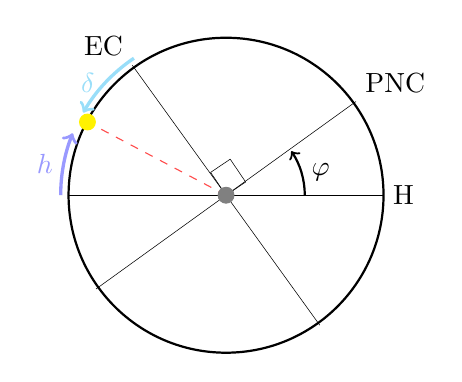
\begin{tikzpicture}
            % Circunferencia
            \draw[black, thick] (0,0) circle (2);
            
            % Rectas / Líneas
            \draw[black, very thin] (-2, 0) -- (2, 0) node[anchor=west]{H};
            \draw[black, very thin] (-1.65, -1.19) -- (1.65, 1.19) node[anchor=south west]{PNC};
            \draw[black, very thin]  (1.19, -1.65) -- (-1.19, 1.65)  node[anchor=south east]{EC};
            % Línea roja
            \draw[red!70, dashed] (0,0) -- (-1.76, 0.93);
        
            % Arcos
            % Declinación
            \draw[cyan!40, very thick, ->] (-1.17, 1.74) arc (124:150:2.1) node[midway, left]{$\delta$};
            % Altura h
            \draw[blue!40, very thick, ->] (-2.1, 0) arc (180:158:2.1) node[midway, left]{$h$};
            \draw[black, thick, ->] (1, 0) arc (0:34:1) node[midway, right]{$\varphi$};
            
            % % Cuadrados
            \draw[black, very thin, rotate around={34:(0,0)}] (0,0) rectangle (0.3, 0.35);
        
            % % Puntos
            \filldraw[fill=black!50, draw=black!50] (0,0) circle (0.1);
            % Estrella a 152º
            \filldraw[fill=yellow, draw=yellow] (-1.76, 0.93) circle (0.1); 
        \end{tikzpicture}
        \caption{$\varphi = \ang{90} + \delta - h$}
    \end{subfigure}
    \hspace{0.1cm}
    \hfill
    \begin{subfigure}{0.3\textwidth}
        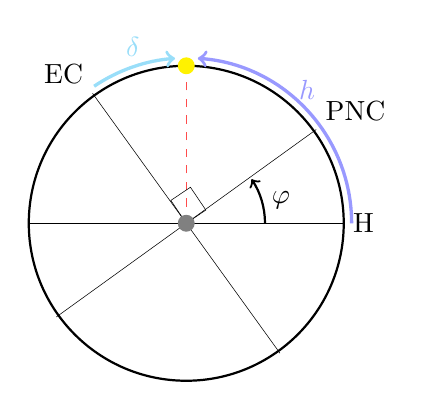
\begin{tikzpicture}
            % Circunferencia
            \draw[black, thick] (0,0) circle (2);
            
            % Rectas / Líneas
            \draw[black, very thin] (-2, 0) -- (2, 0) node[anchor=west]{H};
            \draw[black, very thin] (-1.65, -1.19) -- (1.65, 1.19) node[anchor=south west]{PNC};
            \draw[black, very thin]  (1.19, -1.65) -- (-1.19, 1.65)  node[anchor=south east]{EC};
            % Línea roja
            \draw[red!70, dashed] (0,0) -- (0, 2);
        
            % Arcos
            % Declinación
            \draw[cyan!40, very thick, ->] (-1.17, 1.74) arc (124:94:2.1) node[midway, above]{$\delta$};
            % Altura h
            \draw[blue!40, very thick, ->] (2.1, 0) arc (0:86:2.1) node[midway, above]{$h$};
            \draw[black, thick, ->] (1, 0) arc (0:34:1) node[midway, right]{$\varphi$};
            
            % % Cuadrados
            \draw[black, very thin, rotate around={34:(0,0)}] (0,0) rectangle (0.3, 0.35);
        
            % % Puntos
            \filldraw[fill=black!50, draw=black!50] (0,0) circle (0.1);
            % Estrella a 90º
            \filldraw[fill=yellow, draw=yellow] (0, 2) circle (0.1); 
        \end{tikzpicture}
        \caption{$\varphi = h + \delta -\ang{90}$}
    \end{subfigure}
    % \hspace{0.05cm}
    \hfill
    \begin{subfigure}{0.3\textwidth}
        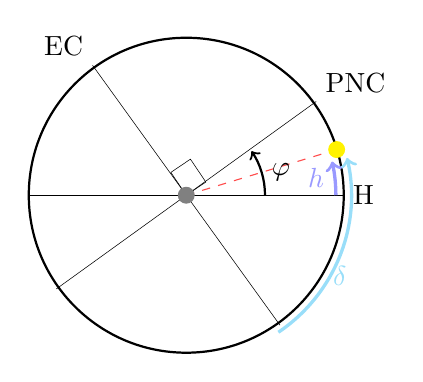
\begin{tikzpicture}
            % Circunferencia
            \draw[black, thick] (0,0) circle (2);
            
            % Rectas / Líneas
            \draw[black, very thin] (-2, 0) -- (2, 0) node[anchor=west]{H};
            \draw[black, very thin] (-1.65, -1.19) -- (1.65, 1.19) node[anchor=south west]{PNC};
            \draw[black, very thin]  (1.19, -1.65) -- (-1.19, 1.65)  node[anchor=south east]{EC};
            % Línea roja
            \draw[red!70, dashed] (0,0) -- (1.91, 0.58);
        
            % Arcos
            % Declinación
            \draw[cyan!40, very thick, ->] (1.17, -1.74) arc (-56:13:2.1) node[midway, below]{$\delta$};
            % Altura h
            \draw[blue!40, very thick, ->] (1.9, 0) arc (0:13:1.9) node[midway, left]{$h$};
            \draw[black, thick, ->] (1, 0) arc (0:34:1) node[midway, right]{$\varphi$};
            
            % % Cuadrados
            \draw[black, very thin, rotate around={34:(0,0)}] (0,0) rectangle (0.3, 0.35);
        
            % % Puntos
            \filldraw[fill=black!50, draw=black!50] (0,0) circle (0.1);
            % Estrella a 17º
            \filldraw[fill=yellow, draw=yellow] (1.91, 0.58) circle (0.1); 
        \end{tikzpicture}
        \caption{$\varphi = \ang{90} + h - \delta$}
    \end{subfigure}  
    \caption{Ecuaciones de latitud en hemisferio norte}
    \label{fig:lat-hemisferio-norte}
\end{figure}


\end{document}